\documentclass[3p]{elsarticle} %preprint/3p

\usepackage{hyperref}

\journal{ }

\usepackage{amsmath} %added for maths environments (equation and align)
\usepackage{amssymb}
\usepackage{upgreek}
\usepackage{bm} %bold symbols by using \bm
\usepackage{mathtools, nccmath} %added for \xrightleftharpoons

\usepackage{subcaption} %allowing for subcaptions and subfigures
\captionsetup[sub]{font=normalsize}%normalsize

\usepackage{algorithm} %added for algorithm box
\usepackage{algpseudocode}

\usepackage[autostyle]{csquotes}
\MakeOuterQuote{"}

\bibliographystyle{elsarticle-num}

% slightly altering rules for figure placement to prevent full-page figures
\usepackage{placeins}
\renewcommand{\floatpagefraction}{.90}
\renewcommand{\topfraction}{.90}

\usepackage[capitalise, nameinlink]{cleveref}

\usepackage{todonotes} %added for todo notes
\let\oldtodo\todo
\renewcommand{\todo}[1]{\oldtodo[inline]{#1}}
%\renewcommand{\todo}[1]{\oldtodo[color=white!40,inline]{#1}}
\newcommand{\toask}[1]{\oldtodo[color=green!40, inline]{#1}}
\newcommand{\wrn}[1]{\oldtodo[color=red!40, inline]{#1}}

\usepackage{xcolor}
\usepackage{listings}
\usepackage{lstautogobble}
\usepackage[numbered]{matlab-prettifier}
\lstdefinestyle{mystyle}{
	numbers=left,
	numberstyle=\footnotesize,
	numbersep=8pt,
	style=Matlab-editor,
	tabsize=4,
	basicstyle=\ttfamily\footnotesize,
	numbersep=25pt,
	frame=none,
	autogobble=true
}

\newcommand{\citeMe}{\href{http://doi.org/XXXX}{T. Hageman \& E. Martínez-Pañeda, \textit{A phase field-based framework for electro-chemo-mechanical fracture: crack-contained electrolytes, chemical reactions and stabilisation}. Computer Methods in Applied Mechanics and Engineering XX (2023) YY} \citep{Hageman2023}}

\begin{document}

\begin{frontmatter}
\title{Physbased Diffusion Embrittlement: a MATLAB code to accurately predict hydrogen embrittlement within the phase-field framework}

\author{Tim Hageman \corref{mycorrespondingauthor}}
\cortext[mycorrespondingauthor]{Corresponding author}
\ead{t.hageman@imperial.ac.uk}
\author{Emilio Martínez-Pañeda}

\address{Department of Civil and Environmental Engineering, Imperial College London, London SW7 2AZ, UK}

\begin{abstract}
Documentation that accompanies the \textit{MATLAB} code \href{https://github.com/T-Hageman/PhysBased_Diffusion_Embrittlement}{Physbased Diffusion Embrittlement, available from \textcolor{blue}{here}}. This documentation explains the usage of the implemented finite element framework, and highlight the main files. Special attention is paid to the parts of the code that implement the physics-based diffusion model for electrolytes within cracks, and how the crack opening height is obtained. 

If using this module for research or industrial purposes, please cite: \citeMe{}.
\todo{update citeMe with correct reference once main paper is published}
\end{abstract}

\begin{keyword}
MATLAB, electrochemistry, phasefield, hydrogen embrittlement, finite element method
\end{keyword}

\end{frontmatter}

\begin{figure}
	\centering
	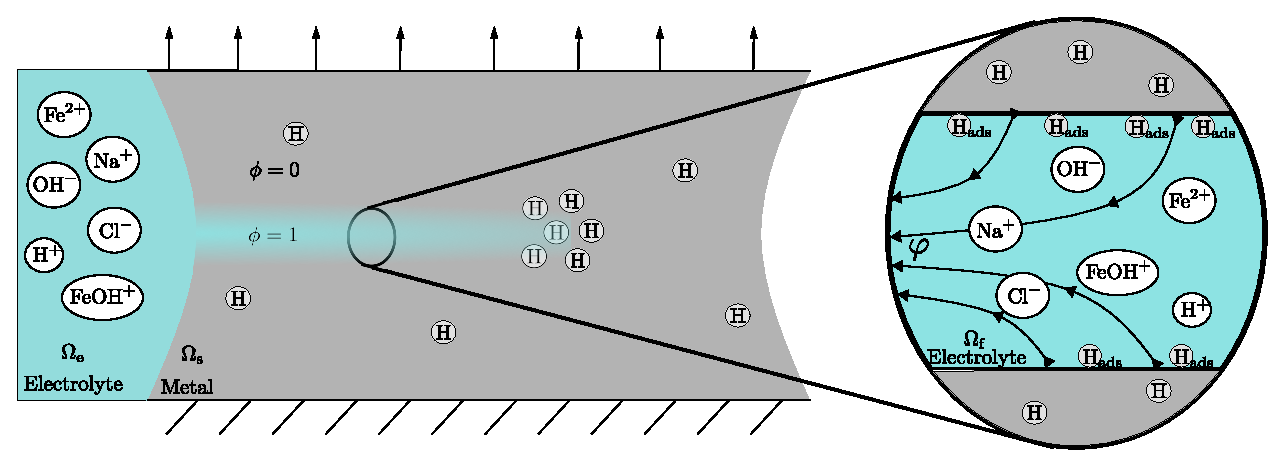
\includegraphics[width=16cm]{Figures/Generic_Domain_DOFs.eps}
	\caption{Overview of the system simulated using the presented MATLAB code}
\end{figure}

\tableofcontents

\section{Introduction}
Development of cracks due to interactions with the environment is a common failure mechanism, with causes of this environment-induced failure including stress-corrosion-cracking and hydrogen embrittlement. Accurately predicting these phenomena does not only require capturing the metal and neighbouring electrolyte, but also requires the effects of newly created and propagating cracks to be captured. One framework enabling crack propagation in arbitrary directions and geometries is the phase field method, representing cracks in a smeared manner. While the mechanical side of phase field fracture models is well-developed, models to represent fluids and species contained within the cracks are usually of a more empirical nature (for instance, requiring fitting parameters that are problem-dependent). Here, we present a MATLAB implementation of a physics-based model for ionic diffusion and reactions within cracks compatible with the phase field framework. This physics-based model is described in \citeMe{}, where its ability to accurately predict hydrogen uptake and expected failure times is shown. In the remainder of this documentation, the physical models and mathematical objects included within this code will be detailed. Special attention is given to the manner in which crack opening heights are reconstructed, as this requires procedures that are non-standard in finite element methods.

Note: as this code is developed along other codes, parts of this code (and the documentation) correspond to the codes accompanying \citep{Hageman2023a} (hydrogen absorption stabilised with lumped integration) and \citep{Hageman2023b} (corrosion under charge conservation conditions).

\subsection{Basic usage}
For simulating the model as provided, running the function "main\_ Static.m" performs all required actions for simulating a static fracture: It automatically generates the geometry and mesh, initialises all simulation components, and prints outputs to the screen and saves them to a folder within results. Simple changes, e.g. editing parameters, can be done within main.m without requiring altering other files. Similarly, "main.m" performs the simulations for a dynamic fracture. Files are also provided for the post-processing: "Animations.m" to generate time-series for the output files, and "compare.m" to plot multiple simulations at a set time.

\section{Summary of included files}
The code is set up in a object-oriented manner, defining matlab classes for each sub-component and providing their accompanying methods. As a result, a clear distinction is made between different components, and each can be used and altered with limited/no impact on other components. Here, the different classes are described. The commenting style employed within the code is compatible with the matlab help function, as such information about all usable methods within a class can be accessed by including the relevant folders, and typing, for instance, "help Solver" to print all variables contained within and all function available from the solver. 

\subsection{main.m}
This is the main file, from which all classes are constructed and the actual simulation is performed. Within it, all properties used within other classes are defined as inputs, for instance for the momentum balance and phase-field evolution equations within the solid domain:
\lstinputlisting[firstnumber=69,firstline=69,lastline=79,style=mystyle,title=main.m]{../main.m}
where "physics{\_}in" is the array of options (in this case, physical models) passed to the physics object at construction. 

The actual time-dependent simulations are also performed within this file:
\lstinputlisting[firstnumber=177,firstline=177,lastline=184,style=mystyle,title=main.m]{../main.m}

Notably, while this performs the time-stepping scheme and controls the time increment size and termination of the simulations, it does not by itself solve anything, instead calling the "solver.Solve()" function which performs a Newton-Raphson procedure using the parameters used to initialize the class, and once the current timestep is converged returns to the main code.

\subsection{Models}
The files included within the Models folder form the main implementation of all the physical phenomena involved. They implement the assembly of tangential matrices and force vectors, when requested by the solving procedures, and store model-specific parameters. 

\subsubsection{BaseModel}
This is an empty model, inherited by all other models to provide consistency within the available functions. While empty within here, the potential functions that can be defined within other models include assembling the system matrix and force vector:
\lstinputlisting[firstnumber=26,firstline=26,lastline=26,style=mystyle,title=Models/@BaseModel/BaseModel.m]{../Models/@BaseModel/BaseModel.m}
and committing history dependent or path dependent variables:
\lstinputlisting[firstnumber=13,firstline=13,lastline=13,style=mystyle]{../Models/@BaseModel/BaseModel.m}
where the keyword "commit{\_}type" indicates the type of history or path dependence to commit at the current point. 
It also provides a function for performing once per staggered solution step actions:
\lstinputlisting[firstnumber=30,firstline=30,lastline=30,style=mystyle]{../Models/@BaseModel/BaseModel.m}


\subsubsection{Constrainer}
This model is used to apply fixed boundary constraints to a degree of freedom at a set location. Within the main file, the inputs required are:
\lstinputlisting[firstnumber=90,firstline=90,lastline=94,style=mystyle,title=main.m]{../main.m}
and multiple definitions of this model are allowed, allowing for constraints to be applied to several element groups. These constraints are integrated within the tangential matrix and force vector through  allocation matrices $\bm{C}_{con}$ and $\bm{C}_{uncon}$, reordering the system into a constrained and unconstrained part. This allows the constrained system to be solved as:
\begin{equation}
	\bm{C}_{uncon}^T \bm{K} \bm{C}_{uncon} \mathbf{y} = -\left(\bm{C}_{uncon}^T\bm{f}+\bm{C}_{uncon}^T \bm{K} \bm{C}_{con}\mathbf{c}\right)
\end{equation}
with the values of the boundary constraints contained in the vector $\mathbf{c}$. After solving, the state vector is then incremented through:
\begin{equation}
	\mathbf{x}^{new} = \mathbf{x}^{old} + \bm{C}_{uncon}\mathbf{y} + \bm{C}_{con}\mathbf{c}
\end{equation}

\subsubsection{LinearElastic}
The linear-elastic model implements the momentum balance for the metal domain:
\begin{equation}
	\bm{\nabla}\cdot\bm{\sigma} = \mathbf{0}
\end{equation}
where the stresses $\bm{\sigma}$ are based on the displacement $\mathbf{u}=["\mathrm{dx}"\;"\mathrm{dy}"]$. The properties used to initialize this model given as input by:
\lstinputlisting[firstnumber=61,firstline=61,lastline=64,style=mystyle,title=main.m]{../mainDiscreteFrac.m}
Notably, since the tangential matrix for linear-elasticity is constant, it is assembled once and saved locally within the model, after which during the global matrix assembly process, it is copied over to the global matrix:
\lstinputlisting[firstnumber=113,firstline=113,lastline=114,style=mystyle,title=Models/@LinearElastic/LinearElastic.m]{../Models/@LinearElastic/LinearElastic.m}
with the force vector also being updated based on this locally saved stiffness matrix. 

\subsubsection{HydrogenDiffusionUnDamaged}
\label{sec:hyd_undamaged}
This model implements the hydrogen mass conservation, through the diffusion equation \citep{Oriani1974, Martinez-Paneda2020, Kristensen2020a, Golahmar2021, Hageman2022}:
\begin{equation}
    \left( 1+\frac{N_\mathrm{T}/N_\mathrm{L} \exp\left(\Delta g_\mathrm{b}/RT\right)}{\left(C_\mathrm{L}/N_\mathrm{L}+\exp\left(\Delta g_\mathrm{b}/RT\right)\right)^2}\right) \dot{C_\mathrm{L}}-\bm{\nabla}\cdot\left(\frac{D_\mathrm{L}}{1-C_\mathrm{L}/N_\mathrm{L}}\bm{\nabla} C_\mathrm{L}\right) + \bm{\nabla} \cdot \left( \frac{D_\mathrm{L} C_\mathrm{L} \overline{V}_\mathrm{H}}{RT}\bm{\nabla}\sigma_\mathrm{H} \right) = 0 \label{eq:hyd_diff}
\end{equation}
with the interstitial lattice hydrogen concentration $C_L$ indicated within the code by "CL". Input properties for this model constitute:
\lstinputlisting[firstnumber=66,firstline=66,lastline=71,style=mystyle,title=mainDiscreteFrac.m]{../mainDiscreteFrac.m}
This model presumes the first model provides the Young's modulus and Poisson ratio. The hydrostatic stress gradients required in this model are obtained as $\bm{\nabla}\sigma_h=\bm{B}_\mathrm{u}^*\mathbf{u}$, with the $\bm{B}^*$ matrix defined as:
\begin{equation}
    \bm{B}_u^* = E/(3(1-2\nu))
    \begin{bmatrix} \frac{\partial^2 N_{u1}}{\partial x^2} & \frac{\partial^2 N_{u2}}{\partial x^2} & \cdot\cdot\cdot & \frac{\partial^2 N_{u1}}{\partial x\partial y} & \frac{\partial^2 N_{u2}}{\partial x\partial y} & \cdot \cdot \cdot \\
    \frac{\partial^2 N_{u1}}{\partial x\partial y} & \frac{\partial^2 N_{u2}}{\partial x \partial y} & \cdot\cdot\cdot & \frac{\partial^2 N_{u1}}{\partial y^2} & \frac{\partial^2 N_{u2}}{\partial y^2} & \cdot \cdot \cdot
    \end{bmatrix}
\end{equation}

\subsubsection{Electrolyte}
The electrolyte model implements the Nernst-Planck mass balance for non-crack contained electrolytes \citep{Planck1890}:
\begin{equation}
    \dot{C}_{\pi}+\bm{\nabla}\cdot\left(-D_\pi \bm{\nabla}C_\pi\right) + \frac{z_\pi F}{RT} \bm{\nabla} \cdot \left(-D_\pi C_\pi \bm{\nabla} \varphi\right) +R_\pi = 0 
\end{equation}
for the ionic species and their name within the model file: $\mathrm{H}^+$ ("H"), $\mathrm{OH}^-$ ("OH"), $\mathrm{Na}^+$ ("Na"), $\mathrm{Cl}^-$ ("Cl", using lower case l; upper case L provides the lattice hydrogen concentration), $\mathrm{Fe}^{2+}$ ("Fe"), and $\mathrm{FeOH}^{+}$ ("FeOH"). Additionally, it implements the electro-neutrality condition \citep{Sarkar2011, Feldberg2000}:
\begin{equation}
	\sum z_\pi C_\pi = 0
\end{equation}
and bulk reactions:
\begin{equation}
    \mathrm{H}_2\mathrm{O} \xrightleftharpoons[k_{w}']{k_{w}} \mathrm{H}^+ + \mathrm{OH}^- \label{react:water}
\end{equation}
\begin{equation}
    \mathrm{Fe}^{2+} + \mathrm{H}_2\mathrm{O} \xrightleftharpoons[k_{fe}']{k_{fe}} \mathrm{FeOH}^+ + \mathrm{H}^+ \label{react:fe_feoh}
\end{equation}
\begin{equation}
    \mathrm{FeOH}^{+} + \mathrm{H}_2\mathrm{O} \xrightharpoonup{k_{feoh}} \mathrm{Fe}(\mathrm{OH})_2 + \mathrm{H}^+ \label{react:feoh_feoh2}
\end{equation}
with reaction rates:
\begin{equation}
    R_{\mathrm{H}^+,w}=R_{\mathrm{OH}^-} = k_{w}C_{\mathrm{H}_2\mathrm{O}} - k_{w}'C_{\mathrm{H}^+}C_{\mathrm{OH}^-}  = k_{eq} \left(K_w-C_{\mathrm{H}^+} C_{\mathrm{OH}^-} \right) \label{eq:water_react}
\end{equation}
\begin{align}
    R_{\mathrm{Fe}^{2+}}&=-k_{fe}C_{\mathrm{Fe}^{2+}}+k_{fe}'C_{\mathrm{FeOH}^+}C_{\mathrm{H}^+} \\
    R_{\mathrm{FeOH}^+}&=k_{fe}C_{Fe^{2+}}-C_{\mathrm{FeOH}^+}(k_{feoh}+k_{fe}'C_{\mathrm{H}^+})\\
    R_{\mathrm{H}^+,fe}&=k_{fe}C_{\mathrm{Fe}^{2+}}-C_{\mathrm{FeOH}^+}(k_{fe}'C_{\mathrm{H}^+}-k_{feoh}) \label{eq:H_Part2}
\end{align}
For this model, the input properties required are:
\lstinputlisting[firstnumber=93,firstline=93,lastline=100,style=mystyle,title=mainDiscreteFrac.m]{../mainDiscreteFrac.m}
This model employs a lumped integration scheme when the vector "Lumped" contains true. Details for the implementation of this lumped scheme are given in \citep{Hageman2023a}.


\subsubsection{ElectrolyteInterface}
The electrolyteInterface model implements the metal-electrolyte coupling through the surface reactions for explicitly represented electrolytes \citep{Liu2014, Hageman2022}:
\begin{alignat}{2}
 \text{Volmer (acid):} && \mathrm{H}^+ + \mathrm{M} + \mathrm{e}^- &\xrightleftharpoons[k_{Va}']{k_{Va}} \mathrm{MH}_{ads} \label{react:1} \\
  \text{Heyrovsky (acid):} && \qquad \mathrm{H}^+ + \mathrm{e}^- + \mathrm{MH}_{ads}&\xrightleftharpoons[k_{Ha}']{k_{Ha}} \mathrm{M} + \mathrm{H}_2 \label{react:2} \\
    \text{Volmer (base):} &&  \mathrm{H}_2\mathrm{O} + \mathrm{M} + \mathrm{e}^- &\xrightleftharpoons[k_{Vb}']{k_{Vb}} \mathrm{MH}_{ads} + \mathrm{OH}^- \label{react:5} \\
   \text{Heyrovsky (base):} && \qquad  \mathrm{H}_2\mathrm{O} + \mathrm{e}^- + \mathrm{MH}_{ads}&\xrightleftharpoons[k_{Hb}']{k_{Hb}} \mathrm{M} + \mathrm{H}_2 + \mathrm{OH}^- \label{react:6} \\
    \text{Tafel:} && 2 \mathrm{MH}_{ads} &\xrightleftharpoons[k_T']{k_T} 2\mathrm{M} + \mathrm{H}_2 \label{react:3} \\
   \text{Absorption:} && \mathrm{MH}_{ads} &\xrightleftharpoons[k_A']{k_A} \mathrm{MH}_{abs}  \label{react:4} \\
   \text{Corrosion:} && \qquad  \mathrm{Fe}^{2+}+2\mathrm{e}^- &\xrightleftharpoons[k_c']{k_c} \mathrm{Fe} \label{react:7}
\end{alignat}
with reaction rates:
\begin{alignat}{4}
\nonumber && && & \qquad\mathrm{Forward} &&  \qquad\qquad \mathrm{Backward} \\
    \mathrm{Volmer (acid):} && \quad && \nu_{Va} &= k_{Va} C_{\mathrm{H}^+}(1-\theta_{ads})e^{-\alpha_{Va} \frac{\eta F}{RT}}\qquad
    && \nu_{Va}' = k_{Va}' \theta_{ads}e^{(1-\alpha_{Va}) \frac{\eta F}{RT}} \label{eq:react1}\\
    \mathrm{Heyrovsky (acid):} && && \nu_{Ha} &= k_{Ha} C_{\mathrm{H}^+}\theta_{ads}e^{-\alpha_{Ha} \frac{\eta F}{RT}}\qquad
    && \nu_{Ha}' = k_{Ha}' (1-\theta_{ads}) p_{\mathrm{H}_2} e^{(1-\alpha_{Ha}) \frac{\eta F}{RT}} \label{eq:react2}\\
    \mathrm{Volmer (base):} && && \nu_{Vb} &= k_{Vb} (1-\theta_{ads})e^{-\alpha_{Vb} \frac{\eta F}{RT}}\qquad
    && \nu_{Vb}' = k_{Vb}' C_{\mathrm{OH}^-} \theta_{ads}e^{(1-\alpha_{Vb}) \frac{\eta F}{RT}} \label{eq:react5}\\
    \mathrm{Heyrovsky (base):} && && \nu_{Hb} &= k_{Hb} \theta_{ads}e^{-\alpha_{Hb} \frac{\eta F}{RT}}\qquad
    && \nu_{Hb}' = k_{Hb}' (1-\theta_{ads}) p_{\mathrm{H}_2} C_{\mathrm{OH}^-} e^{(1-\alpha_{Hb}) \frac{\eta F}{RT}}  \label{eq:react6}\\
    \mathrm{Tafel:} && && \nu_T &= k_T\left|\theta_{ads}\right|\theta_{ads}\qquad
    && \nu_T' = k_T' (1-\theta_{ads})p_{\mathrm{H}_2} \label{eq:react3}\\
    \mathrm{Absorption:} && && \nu_A &= k_A (N_L - C_L)\theta_{ads}\qquad
    && \nu_A' = k_A' C_L (1-\theta_{ads}) \label{eq:react4}\\
    \mathrm{Corrosion:} && && \nu_{c} &= k_{c} C_{\mathrm{Fe}^{2+}}e^{-\alpha_{c} \frac{\eta F}{RT}} \qquad && \nu_{c}' = k_{c}' e^{(1-\alpha_{c}) \frac{\eta F}{RT}}   \label{eq:react7}
\end{alignat}
These reaction rates are implemented in a separate function from the matrix assembly:
\lstinputlisting[firstnumber=392,firstline=392,lastline=392,style=mystyle,title=Models/@ElectrolyteInterface/ElectrolyteInterface.m]{../Models/@ElectrolyteInterface/ElectrolyteInterface.m}
which takes the local hydrogen, hydroxide, and iron concentrations, the surface coverage, electrolyte potential, and interstitial lattice hydrogen concentration. It functions for both the integration-point variables as well as for the nodal values. In addition to the reaction rates, the electrolyte interface model also resolves the surface mass balance:
\begin{equation}
    N_{ads} \dot{\theta}_{ads} - (\nu_{Va}-\nu_{Va}') + \nu_{Ha} + 2 \nu_T + (\nu_A-\nu_A') - (\nu_{Vb}-\nu_{Vb}') + \nu_{Hb} = 0
\end{equation}
For this model, the input variables to define are given as:
\lstinputlisting[firstnumber=102,firstline=102,lastline=108,style=mystyle,title=mainDiscreteFrac.m]{../mainDiscreteFrac.m}
\lstinputlisting[firstnumber=9,firstline=9,lastline=15,style=mystyle]{../mainDiscreteFrac.m}
with the vector "Lumped" allowing for individual interface reactions to be either integrated using a standard Gauss integration scheme (0) or a lumped integration scheme (1). the reaction constants matrix k is defined as:
\begin{equation}
	k = \begin{bmatrix} 
	k_{Va} & k_{Va}' & \alpha_{Va} & E_{eq,Va} \\ 
	k_{Ha} & k_{Ha}' & \alpha_{Ha} & E_{eq,Ha} \\ 
	k_{T} & k_{T}' & - & - \\ 
	k_{A} & k_{A}' & - & - \\ 
	k_{Vb} & k_{Vb}' & \alpha_{Vb} & E_{eq,Vb} \\ 
	k_{Hb} & k_{Hb}' & \alpha_{Hb} & E_{eq,Hb} \\ 
	k_{c} & k_{c}' & \alpha_{c} & E_{eq,c} \\ 
	\end{bmatrix} \label{eq:kmat}
\end{equation}
with the empty entries not used within the model.

\subsubsection{PhasefieldDamage}
This model implements the momentum conservation for a damaged linear-elastic material:
\begin{equation}
    0 = \bm{\nabla}  \cdot \left(d(\phi) \frac{\partial \psi_\mathrm{0}}{\partial \bm{\varepsilon}}\right)  \label{eq:mom}
\end{equation}
and the phase-field evolution equation \citep{Miehe2010,Miehe2010a,Borden2012,Wu2016}:
\begin{equation}
    \frac{\phi}{\ell} - \ell \bm{\nabla}^2\phi = - \frac{\partial d(\phi)}{\partial \phi} \mathcal{H} \qquad \mathrm{where} \qquad \mathcal{H} = \frac{\psi_\mathrm{0}}{G_\mathrm{c}(C_\mathrm{L})}, \; \, \dot{\mathcal{H}}>=0
    \label{eq:phasefieldEvolution}
\end{equation}
using the linear-elastic energy function for an undamaged material:
\begin{equation}
\psi_0 = \mathbf{\varepsilon}:\mathcal{D}:\mathbf{\varepsilon}
\end{equation}
and the damage function:
\begin{equation}
    d(\phi) = k_\mathrm{0} + (1-k_\mathrm{0}) (1-\phi)^2 \label{eq:degradeFunction}
\end{equation}
Within this model, the displacement and phase-field damage variable can not be updated at the same time, instead requiring \cref{eq:mom,eq:phasefieldEvolution} to be set to different staggered solver steps. The history field required within this model is calculated each time the tangent matrix is assembled:
\lstinputlisting[firstnumber=275,firstline=275,lastline=287,style=mystyle,title=Models/@PhaseFieldDamage/PhaseFieldDamage.m]{../Models/@PhaseFieldDamage/PhaseFieldDamage.m}
and changes are committed to the new time increments once the phsics object calls its "Commit" function.

For the initialization of the phase-field parameter, an estimated history field is set via:
\begin{equation}
    \phi^{\mathrm{init}} = \exp\left(-\left|\text{d}x\right|/\ell\right) 
    \qquad \qquad 
    \mathcal{H}^{\mathrm{init}} = \frac{1/\ell \; \; \mathbf{N}_\phi \bm{\upphi}^{\mathrm{init}} + \ell \left(\bm{\nabla}\mathbf{N}_\phi \bm{\upphi}^{\mathrm{init}}\right)^T\left(\bm{\nabla}\mathbf{N}_\phi \bm{\upphi}^{\mathrm{init}}\right)}{k_\mathrm{0}-2(1-k_{\mathrm{0}})\left(1-\mathbf{N}_{\phi}\bm{\upphi}^{\mathrm{init}}\right)} \label{eq:initialization}
\end{equation}
the first time the "OncePerStep" function is called:
\lstinputlisting[firstnumber=97,firstline=97,lastline=148,style=mystyle,title=Models/@PhaseFieldDamage/PhaseFieldDamage.m]{../Models/@PhaseFieldDamage/PhaseFieldDamage.m}
As can be seen, this initial field is set based on the fracture length "Lfrac", and inserted in the centre of the domain. 

Input parameters that need to be set for this model are:
\lstinputlisting[firstnumber=69,firstline=69,lastline=79,style=mystyle,title=main.m]{../main.m}

\subsubsection{HydrogenDiffusion}
Similar to the model presented in \cref{sec:hyd_undamaged} for hydrogen diffusion in undamaged materials, this model simulates the diffusion in damaged materials. While the governing equations displayed in \cref{eq:hyd_diff} are still being simulated, the hydrostatic stress gradient is now interacts with the phase-field damage as:
\begin{equation}
	\nabla\sigma_h = \frac{E}{3(1-2\nu)}\left(d(\phi)\bm{B}^*\mathbf{u}+\frac{\partial d(\phi)}{\partial \phi} \nabla \phi \overline{\bm{B}} \mathbf{u} \right)
\end{equation}
where
\begin{equation}
\overline{\bm{B}} = 
\begin{bmatrix}
	\frac{\partial N_{u1}}{\partial x} & \frac{\partial N_{u1}}{\partial x} & \cdot \cdot \cdot \frac{\partial N_{u1}}{\partial y} & \frac{\partial N_{u1}}{\partial y} & \cdot \cdot \cdot
\end{bmatrix}
\end{equation}

Input parameters required for this model are:
\lstinputlisting[firstnumber=81,firstline=81,lastline=88,style=mystyle,title=main.m]{../main.m}

\subsubsection{PhasefieldElectrolyte}
\label{sec:CrackElectrolyte}
This model simulates the Nernst-Planck and electroneutrelity equations, surface adsorbed hydrogen concentration, and bulk and volume reactions for a crack-contained electrolyte. This system is described by:
\begin{align}
    0 &= \beta_\mathrm{c} \dot{C}_{\pi} - \bm{\nabla} \cdot \left(\bm{R}^T\bm{\beta_\mathrm{d}}\bm{R} D_{\pi} \bm{\nabla} C_\pi \right) - \frac{z_\pi F}{RT}\bm{\nabla} \cdot \left(\bm{R}^T\bm{\beta_\mathrm{d}}\bm{R} D_{\pi} C_\pi \bm{\nabla} \varphi \right) + \beta_\mathrm{c} R_\pi  + \beta_\mathrm{s} \nu_\pi \label{eq:electrolyte_nernstplanck}\\
    0 &= \beta_\mathrm{c} \sum_\pi z_\pi C_\pi \label{eq:electrolyte_neutrality} \\
    0 & =\beta_\mathrm{s} \left(N_{\mathrm{ads}} \dot{\theta}_{\mathrm{ads}} - (\nu_{\mathrm{Va}}-\nu_{\mathrm{Va}}') + \nu_{\mathrm{Ha}} + 2 \nu_\mathrm{T} + (\nu_\mathrm{A}-\nu_\mathrm{A}') - (\nu_{\mathrm{Vb}}-\nu_{\mathrm{Vb}}') + \nu_{\mathrm{Hb}}\right) \label{eq:electrolyte_surface}
\end{align}
The capacity, diffusion, and surface distributors are accordingly defined as:
\begin{alignat}{3}
\nonumber & \mathbf{Distributed}\; \mathbf{diffusion} &&  \qquad\qquad && \mathbf{Physics}\mathbf{-}\mathbf{based} \\
&\beta_\mathrm{c} = \phi^m && && \beta_\mathrm{c} = h \left( \frac{1}{2\ell}\phi^2+\frac{\ell}{2}\left|\bm{\nabla} \phi \right|^2 \right) \label{eq:betac} \\
&\bm{\beta}_\mathrm{d} = \begin{bmatrix} \phi^m D_{\pi,2}/D_\pi & 0\\ 0 & 0 \end{bmatrix} && && \bm{\beta}_\mathrm{d} = \left( \frac{1}{2\ell}\phi^2+\frac{\ell}{2}\left|\bm{\nabla} \phi \right|^2 \right) \begin{bmatrix} h & 0\\ 0 & D_{\infty} \end{bmatrix} \\
&\beta_\mathrm{s} = \frac{1}{\ell}\phi^2+\ell\left|\bm{\nabla} \phi \right|^2  && && \beta_\mathrm{s} = \frac{1}{\ell}\phi^2+\ell\left|\bm{\nabla} \phi \right|^2 \label{eq:betas}
\end{alignat}
where the distribution method is set within the code to either "WuLorenzis" for the distributed diffusion model described in \citep{Wu2016} or "Subgrid" for the physics-based model from this work \citep{Hageman2023}. The manner in which the crack opening height is obtained is described in detail in \cref{sec:OpeningHeights}. 

Input parameters for this model are:
\lstinputlisting[firstnumber=108,firstline=108,lastline=130,style=mystyle,title=main.m]{../main.m}
where the surface reaction rates $k_{surf}$ follows the format from \cref{eq:kmat}. This model also implements post-processing functions specifically for the electro-chemical system contained within the crevasse:
\lstinputlisting[firstnumber=795,firstline=795,lastline=795,style=mystyle,title=Models/@PhaseFieldElectrolyte/PhaseFieldElectrolyte.m]{../Models/@PhaseFieldElectrolyte/PhaseFieldElectrolyte.m}
which plots the crack opening height and the crack-normal vectors,
\lstinputlisting[firstnumber=833,firstline=833,lastline=833,style=mystyle]{../Models/@PhaseFieldElectrolyte/PhaseFieldElectrolyte.m}
plotting electrolyte concentrations and the electrolyte potential, and
\lstinputlisting[firstnumber=894,firstline=894,lastline=894,style=mystyle]{../Models/@PhaseFieldElectrolyte/PhaseFieldElectrolyte.m}
plotting the pH of the electrolyte. This last function solely show results where $\phi>0.1$, filtering out the non-physical state of the electrolyte.

\subsection{Mesh}
This class contains the nodes and elements that describe the geometry, and provides support for evaluating shape functions. Within its implementation, it uses a multi-mesh approach, defining element groups for each entity within the domain (for instance, defining an element group "Interior" for the metal domain composed of surface elements, and defining an element group "Interface" composed of line elements which coincide with the electrolyte-metal interface). The geometry of the problem is defined through procedures within the mesh class.

The mesh class also provides a direct interfaces from which to get the element shape functions, second gradients, and surface-normal vectors, providing an element group number and the index of the element itself:
\lstinputlisting[firstnumber=19,firstline=19,lastline=21,style=mystyle,title=@Mesh/mesh.m]{../@Mesh/Mesh.m}
which returns a matrix containing the shape functions N within all integration points of the element, gradients of the shape function G, and the integration weights for all integration points w. Additionally, for the construction of the hydrogen diffusion model, the second-order gradients G2 are provided through a separate function.

\subsection{Shapes}
The classes within this folder provide basic shape functions, and are used by the mesh to provide shape functions and integration weights. The included shape functions are square Lagrangian and triangular Bernstein surface elements (Q9 and T6), quadratic Lagrangian and Bernstein line elements (L3 and L3B), and interface elements (LI6, unused).

\subsection{Physics}
This class provides all the support required for constructing and managing state and force vectors, tangential matrices, and boundary constraints. Most notably, during its initialization it generates an array of all the physical models, from which it then is able to construct the tangential matrix when required:
\lstinputlisting[firstnumber=63,firstline=63,lastline=83,style=mystyle,title=@Physics/Physics.m]{../@Physics/Physics.m}
This calls each of the models, and passes a handle to the physics object itself through which the individual models can add their contributions. Notably, the force vector and tangent matrix being assembled by this function are those associated with the staggered solver step "stp", with this step index being passed onto the individual models, which then either add their contributions to the tangent matrix or do not undertake nay action. In a similar manner, actions which should be performed once at the start of each staggered solution step are performed via:
\lstinputlisting[firstnumber=54,firstline=54,lastline=60,style=mystyle,title=@Physics/Physics.m]{../@Physics/Physics.m}

The physics class also provides the ability for post-processing the results through the function;
\lstinputlisting[firstnumber=26,firstline=26,lastline=27,style=mystyle,title=@Physics/Physics.m]{../@Physics/Physics.m}
This function requires the name of a degree of freedom (for instance "dx" for the horizontal displacements, or "H" for the hydrogen ion concentration), a scale to indicate whether the mesh is plotted in deformed (scale$>$0) or undeformed (scale$=$0) configuration, and the name of an element group on which to plot the results. Similarly, the "PlotIP" function plots integration-point specific variables, for instance stresses or history fields.

\subsection{Dofspace}
This class converts the node numbering, degree of freedom type, and solution step to an index for the degree of freedom, corresponding to its location within the unconstrained state vector and tangential matrix. Specific types of degree of freedom are registered on initialization of the dofspace through:
\lstinputlisting[firstnumber=17,firstline=17,lastline=27,style=mystyle,title=@DofSpace/DofSpace.m]{../@DofSpace/DofSpace.m}
For the numbering scheme saved within "DofNumbering", each solution step retains its own numbering. 

After initializing the dofspace, degrees of freedom can be added to nodes through:
\lstinputlisting[firstnumber=29,firstline=29,lastline=31,style=mystyle]{../@DofSpace/DofSpace.m}
These functions automatically check for duplicates, such that each model can safely add all the degrees of freedom relevant to itself, without taking into account potential interactions with other models. During the finite element assembly, the managed degrees of freedom indices are requestable by providing the degree of freedom type index and the node number:
\lstinputlisting[firstnumber=68,firstline=68,lastline=71,style=mystyle]{../@DofSpace/DofSpace.m}
which assumes the model already knows which staggered solver step the degree of freedom is associated with. These solver step indices can also be requested through:
\lstinputlisting[firstnumber=51,firstline=51,lastline=53,style=mystyle]{../@DofSpace/DofSpace.m}
which takes the name of the degree of freedom, and returns its index and the staggered step (and thus state vector) associated with this degree of freedom.

\subsection{Solver}
\begin{algorithm}[t]
\caption{Overview of solution method}\label{alg:solution_scheme}
\begin{algorithmic}[1]
\State Start of time increment
\While{not converged}
\State Step 1: Update $\bm{\upphi}$
\State Step 2: Update $\mathbf{u}$
\State Perform OncePerStep 3: Update $h$
\While{$\mathbf{C}_\mathrm{L}$, $\mathbf{C}_\pi$, $\bm{\upvarphi}$, $\bm{\uptheta}$ are not converged}
    \State Step 3: update $\mathbf{C}_\mathrm{L}$, $\mathbf{C}_\pi$, $\bm{\upvarphi}$, $\bm{\uptheta}$
    \State Calculate energy based residual for $\mathbf{C}_\mathrm{L}$, $\mathbf{C}_\pi$, $\bm{\upvarphi}$, $\bm{\uptheta}$
\EndWhile
    \State Calculate energy based residual for $\mathbf{u}$ and $\bm{\upphi}$
\EndWhile
\State Go to next time increment
\end{algorithmic}
\end{algorithm}
The solver class implements a iteratively staggered Newton-Raphson type nonlinear solver, including the ability to perform linear line-searches to improve the convergence rate and stability. During its creation, it gets linked to the physics object, such that it can automatically request updated tangential matrices. An example of the staggered solution scheme solved through this solver is shown in Algorith \ref{alg:solution_scheme}. Input parameters controlling the solver behaviour are:
\lstinputlisting[firstnumber=138,firstline=138,lastline=144,style=mystyle,title=main.m]{../main.m}

\section{Specifics: Fracture opening height}
\label{sec:OpeningHeights}
\begin{figure}
	\centering
	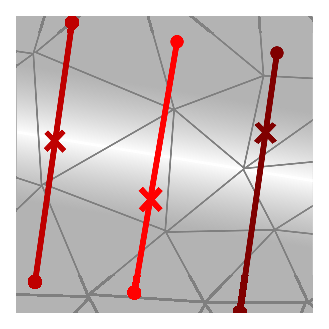
\includegraphics{Figures/Example_OpeningHeight.eps}
	\caption{Schematic overview of integrations performed to calculate the crack opening height}
	\label{fig:OpeningHeightsFig}
\end{figure}

Within the model for the crack-contained electrolyte, \cref{sec:CrackElectrolyte}, the estimated opening height of the crevasse is needed. These opening heights are calculated through an integral normal to the fracture surface \citep{Yoshioka2020, Chukwudozie2019}:
\begin{equation}
    h = \int \mathbf{u}\cdot\bm{\nabla}\phi \; \mathrm{d}n \label{eq:heightmapping}
\end{equation}
with the line along which this integral is performed shown in \cref{fig:OpeningHeightsFig}, and the normal vector based on the phase-field as:
\begin{equation}
    \bm{n} = \frac{\bm{\nabla}\phi}{\left|\bm{\nabla}\phi\right|}
\end{equation}

These integrals are implemented in:
\lstinputlisting[firstnumber=196,firstline=196,lastline=203,style=mystyle,title=Models/@PhaseFieldElectrolyte/PhaseFieldElectrolyte.m]{../Models/@PhaseFieldElectrolyte/PhaseFieldElectrolyte.m}
which fills the "Height" and "normals" matrices with the opening heights and normal vectors for all elements and all integration points. This function is only called once per staggered iteration step, as the phase-field and displacements are assumed to stay constant during the electro-chemical solution step. 

First, the displacements and gradients within all integration points are determined:
\lstinputlisting[firstnumber=205,firstline=205,lastline=233,style=mystyle,title=Models/@PhaseFieldElectrolyte/PhaseFieldElectrolyte.m]{../Models/@PhaseFieldElectrolyte/PhaseFieldElectrolyte.m}
and these opening heights are used to construct interpolation functions:
\lstinputlisting[firstnumber=235,firstline=235,lastline=244,style=mystyle,title=Models/@PhaseFieldElectrolyte/PhaseFieldElectrolyte.m]{../Models/@PhaseFieldElectrolyte/PhaseFieldElectrolyte.m}
These interpolation functions are then used to construct an interpolation function for the crack opening height based on \cref{eq:heightmapping}, for instance when the crack path is solely horizontal:
\lstinputlisting[firstnumber=246,firstline=246,lastline=255,style=mystyle,title=Models/@PhaseFieldElectrolyte/PhaseFieldElectrolyte.m]{../Models/@PhaseFieldElectrolyte/PhaseFieldElectrolyte.m}
and finally the crack opening heights and normal vectors within integration points are produced as:
\lstinputlisting[firstnumber=269,firstline=269,lastline=287,style=mystyle,title=Models/@PhaseFieldElectrolyte/PhaseFieldElectrolyte.m]{../Models/@PhaseFieldElectrolyte/PhaseFieldElectrolyte.m}
It should be noted that this does not produce opening heights which exactly match to the expected opening based on the displacement and phase-field. However, as long as enough intermediate points are used (e.g. the 1000 points declared on line 248), these results will be virtually indistinguishable from the opening heights that could be calculated by evaluating the phase-field gradient and displacements exactly. The implementation presented here furthermore does not take into account branching cracks, instead assuming the phase-field tends towards zero away from the crack interface.

\section{Sample results}

\subsection{Static cracks}
\begin{figure}
	\centering
	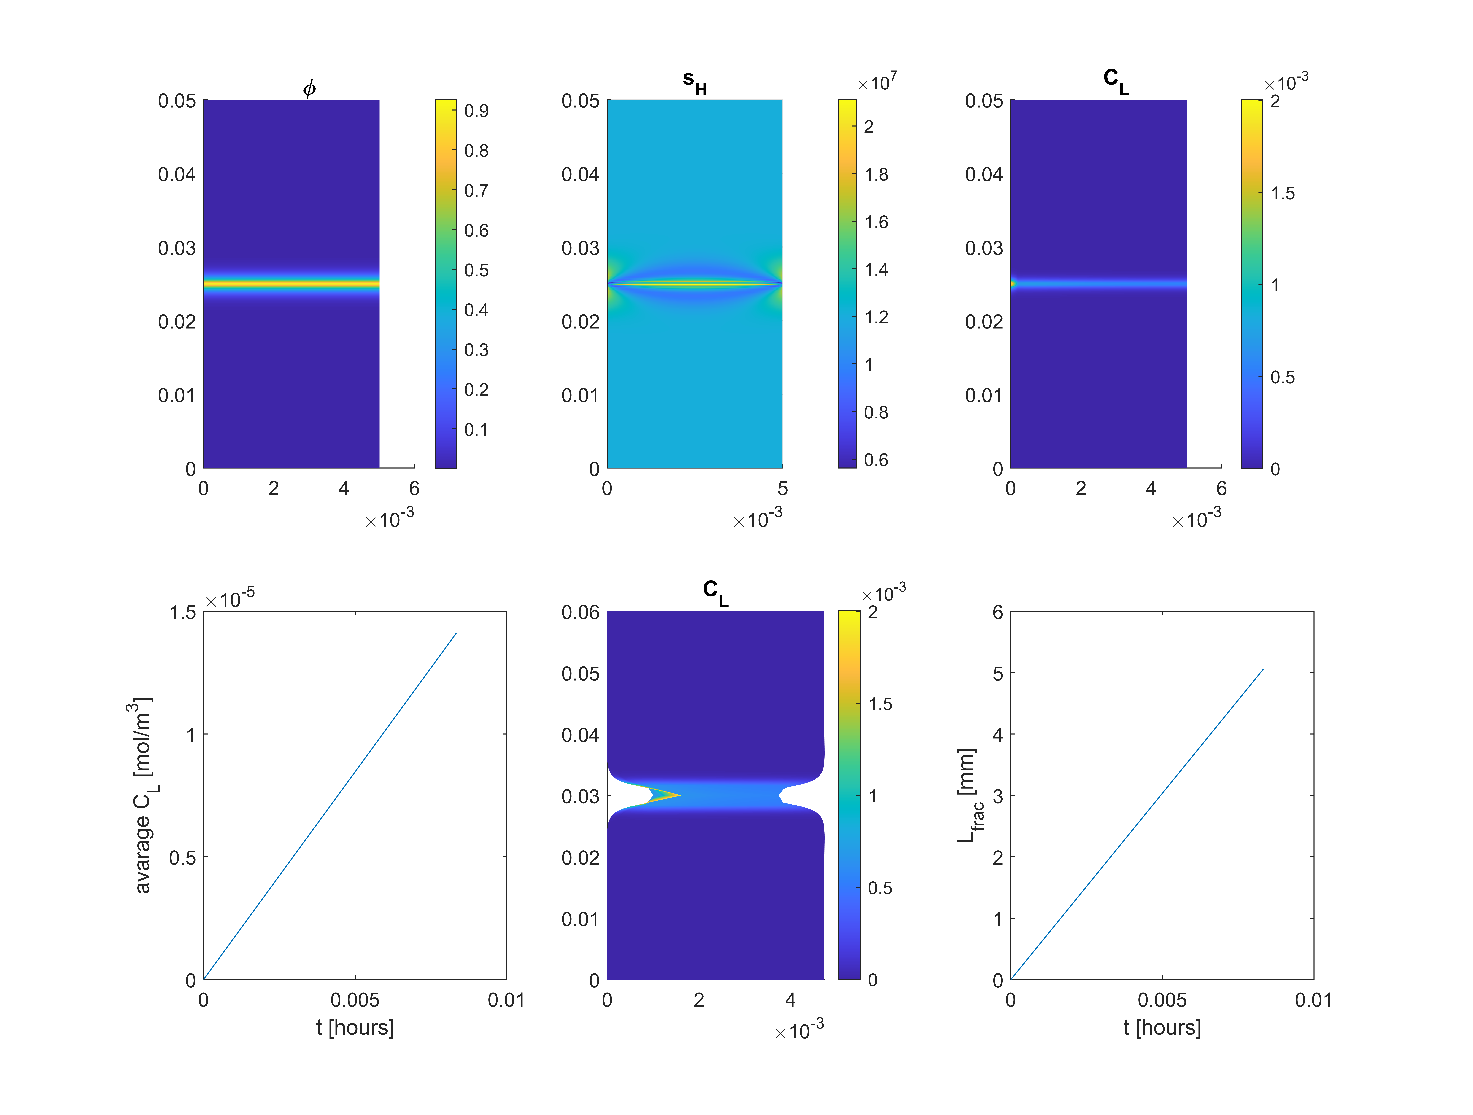
\includegraphics[width=16cm]{./Figures/Res_Static2.eps}
	\caption{Results produced by running "main{\_}Static("Subgrid", 5e-4, 1e-5)". The first row shows the phase field, hydrostatic stress, and interstitial lattice hydrogen concentration. The second row shows the avarage hydrogen uptake over time, interstitial lattice concentration in the deformed configuration, and fracture length over time.}
	\label{res1}
\end{figure}
\begin{figure}
	\centering
	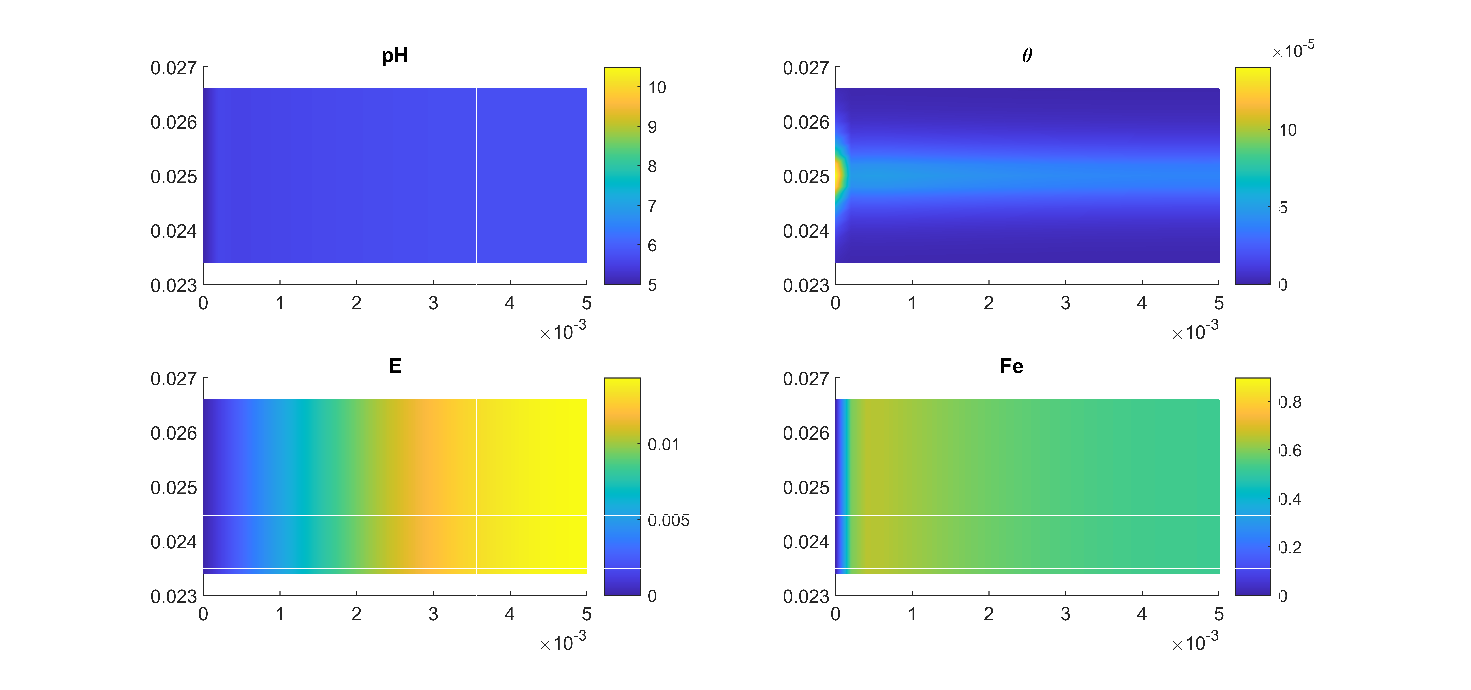
\includegraphics[width=12cm]{./Figures/Res_Static1.eps}
	\caption{Results produced by running "main{\_}Static("Subgrid", 5e-4, 1e-5)", showing the electrolyte pH, surface adsorbed hydrogen concentration, electrolyte potential and $\mathrm{Fe}^{2+}$ concentration.}
	\label{res2}
\end{figure}
For verification cases using a static crack, a single simulatioin can be run via "main{\_}Static(model, l, u)", where model is either "Subgrid" or "WuLorenzis" for the physics-based or distributed diffusion models, l is the phase-field length scale, and u is the displacement (for instance, running "main{\_}Static("Subgrid", 5e-4, 1e-5)"). Once running, a folder is created in "./Results{\_}NoProp/" where output data is saved, and results are plotted after each converged time increment. Results after the first time increment are shown in \cref{res1,res2}. 

In addition to running a single case, the file "DoSweep.m" performs a parametric sweep over the two models, and several external displacements and phase field length scales. It also runs simulations for a discrete representation of the crack, and creates a figure showing the comparison between the models. please note, as this function runs quite a few simulations, it takes a while to run fully.


\subsection{Propagating cracks}
\begin{figure}
	\centering
	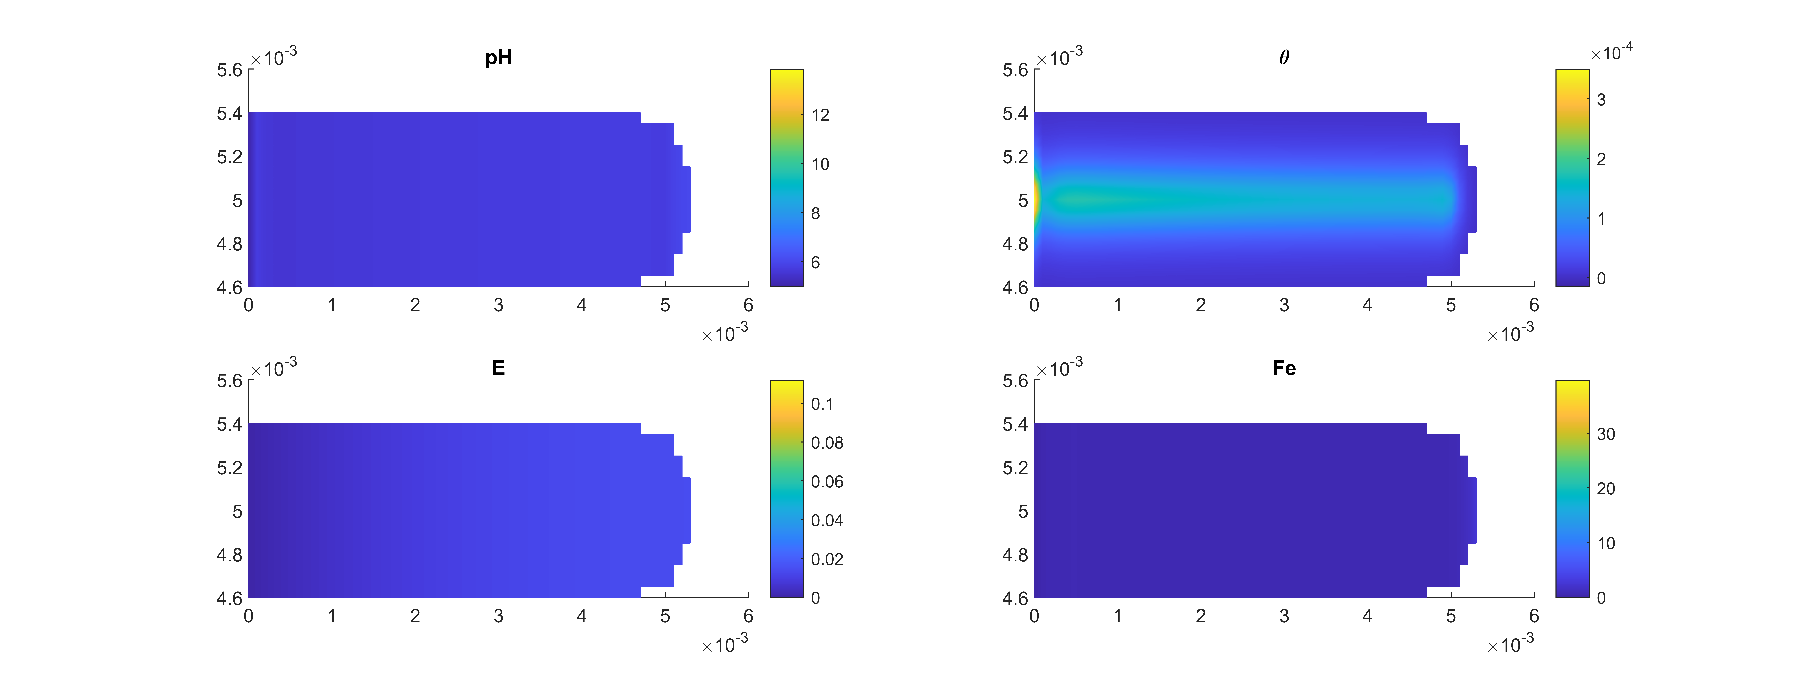
\includegraphics[width=16cm]{./Figures/Res_Static4.eps}
	\caption{Results produced by running "main(1)". The first row shows the phase field, hydrostatic stress, and interstitial lattice hydrogen concentration. The second row shows the avarage hydrogen uptake over time, interstitial lattice concentration in the deformed configuration, and fracture length over time.}
	\label{res3}
\end{figure}
\begin{figure}
	\centering
	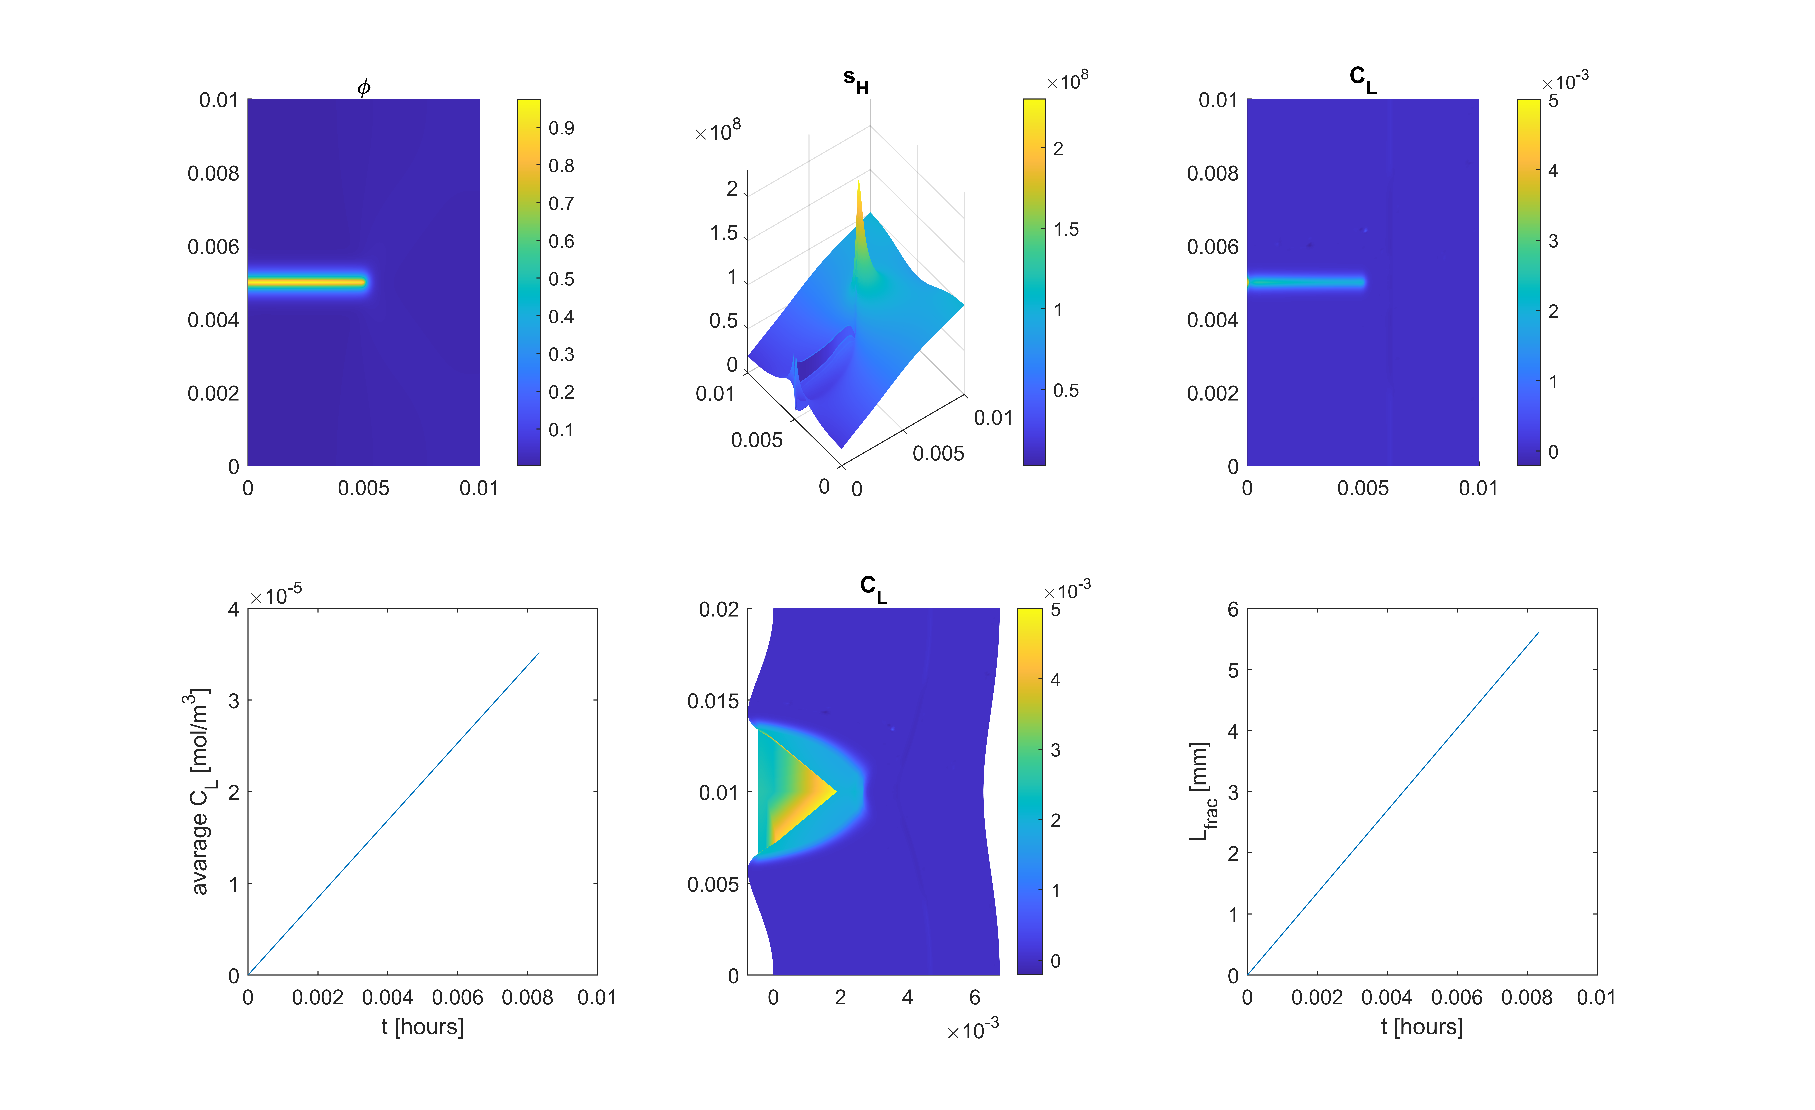
\includegraphics[width=12cm]{./Figures/Res_Static3.eps}
	\caption{Results produced by running "main(1)", showing the electrolyte pH, surface adsorbed hydrogen concentration, electrolyte potential and $\mathrm{Fe}^{2+}$ concentration.}
	\label{res4}
\end{figure}
The function "main.m" performs a simulation of a propagating crack in a square plate, using the parameters set in this main file. Please note that this function takes a while to run. Results after the first time increment are shown in \cref{res3,res4}. 

\bibliography{references}

\end{document}
